%!TEX root = slides.tex

\title{Theory of Algorithms}
\subtitle{}
\author{ian.mcloughlin@gmit.ie}
\date{}


\begin{frame}
	\titlepage
\end{frame}

\begin{frame}
	\frametitle{Topics}
	\tableofcontents
\end{frame}

\section{Python}


\begin{frame}{About Python}
  \begin{description}
    \item[January 1994] -- Python 1.0.0 released.
    \vspace{0.25cm}
    \item[Guido van Rossum] -- Designer/Author of Python.
    \vspace{0.25cm}
    \item[Current versions] -- 3.5.1 and 2.7.11.
    \vspace{0.25cm}
    \item[Interpreted] -- Python implementation must be present at runtime.
    \vspace{0.25cm}
    \item[Off-side rule] -- Blocks identified by indentation, as opposed to curly braces.
    \vspace{0.25cm} 
    \item[Popularity] -- IEEE Spectrum ranks it as the fourth most popular language (July 2015).
    \vspace{0.25cm}
    \item[Community] -- Python Enhancement Proposals, notably \href{https://www.python.org/dev/peps/pep-0008/}{PEP 8: The Python Style Guide}.
    \vspace{0.25cm} 
  \end{description}
  \citeurl{spectrum.ieee.org/computing/software/the-2015-top-ten-programming-languages}
\end{frame}


\begin{frame}{Guido van Rossum}
  \begin{columns}
    \begin{column}{0.2\textwidth}
      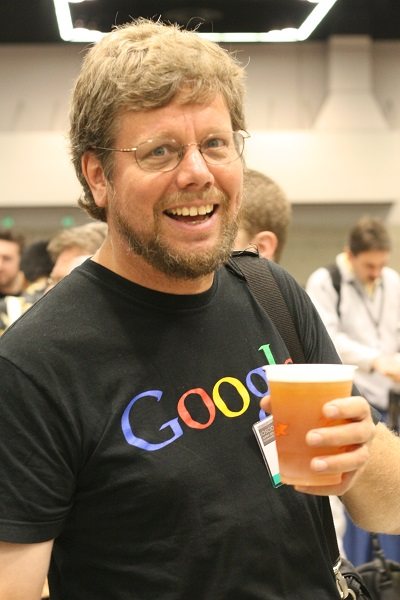
\includegraphics[height=2in]{img/guido_van_rossum.jpg}
    \end{column}
    \begin{column}{0.6\textwidth}
      \begin{itemize}
    		\item Started Python as a hobby.
        \vspace{0.25cm}
    		\item Worked for Google, half-time spent on Python.
        \vspace{0.25cm}
    		\item Now works at Dropbox.
        \vspace{0.25cm}
        \item Benevolent dictator for life (BDFL).
      \end{itemize}
    \end{column}
  \end{columns}
\end{frame}

\begin{frame}[fragile]{Conditions}
  \begin{minted}[linenos, frame=lines, framesep=2mm]{python}
x = int(raw_input("Please enter an integer: "))
if x < 0:
  x = 0
  print 'Negative changed to zero'
elif x == 0:
  print 'Zero'
elif x == 1:
  print 'Single'
else:
  print 'More'
  \end{minted}
  \citeurl{docs.python.org/2/tutorial}
\end{frame}

\begin{frame}[fragile]{Loops}
  \begin{minted}[linenos, frame=lines, framesep=2mm]{python}
# A for loop.
a = ['Mary', 'had', 'a', 'little', 'lamb']
for i in range(len(a)):
  print(i, a[i])
  \end{minted}
  \begin{minted}[linenos, frame=lines, framesep=2mm]{python}
# A while loop.
a, b = 0, 1
while b < 1000:
  print(b)
  a, b = b, a+b
  \end{minted}
  \citeurl{docs.python.org/3/tutorial}
\end{frame}

\begin{frame}[fragile]{Functions}
  \begin{minted}[linenos, frame=lines, framesep=2mm]{python}
# write Fibonacci series up to n
def fib(n):   
  """Print a Fibonacci series up to n."""
  a, b = 0, 1
  while a < n:
    print(a)
    a, b = b, a+b
  \end{minted}
  \citeurl{docs.python.org/3/tutorial}
\end{frame}

\begin{frame}{CPython}
  \begin{description}
    \item[Reference implementation] -- Many different Python implementations exist.
    \vspace{0.25cm}
    \item[Version 3] -- Broke backwards compatibility (somewhat).
    \vspace{0.25cm}
    \item[Unladen Swallow] -- Google attempt to fix some Python problems.
    \vspace{0.25cm}
    \item[Modules] -- Lots of great Python modules available.
  \end{description}
  \citeurl{www.python.org}
\end{frame}

\begin{frame}[fragile]{Lists}
	\begin{description}
		\item[Lists] in Python are usually written as comma-separated values between square brackets.
		\item[Types] -- elements of a list don't have to have the same types.
		\item[Slicing] is possible, where we take a sublist of the list.
		\item[Assignment] to slices is possible.
		\item[len()] is a built-in function that returns the length of a list.
		\item[range()] is a built-in function that returns a list of numbers. Note: it returns an \emph{iterator}.
	\end{description}
	\begin{minted}[linenos, frame=lines, framesep=2mm]{python}
letters = ['a', 'b', 'c']
letters[1:] = ['c', 'd']
range(10) # [0,1,2,3,4,5,6,7,8,9]
  \end{minted}
  \citeurl{docs.python.org/3/tutorial}
\end{frame}

\begin{frame}[fragile]{Strings}
	\begin{description}
	  \item[Strings] are a lot like lists in Python.
	  \item[Assignment] to slices is not allowed, however.
	\end{description}
	\begin{minted}[linenos, frame=lines, framesep=2mm]{python}
words = "This is a sentence."
words[8]         # a
words[5:7]       # is
words[:7]        # This is
words[10:]       # sentence.
words[17:9:-1]   # ecnetnes

len(words)       # 19
"One" + "Two"    # OneTwo
  \end{minted}
	\citeurl{docs.python.org/3/tutorial}
\end{frame}

\begin{frame}[fragile]{Functions}
	\begin{description}
	  \item[def] is the keyword for defining a function.
	  \item[Parameters] can be given defaults, so that they are optional.
	\end{description}
	\begin{minted}[linenos, frame=lines, framesep=2mm]{python}
def axn(x, a=1, n=2):
	return a*(x**n)    # ax^n
 
axn(3)       # 9
axn(3, 2)    # 18
axn(3, 2, 3) # 54
axn(3, n=3)  # 27
  \end{minted}
	\citeurl{docs.python.org/3/tutorial}
\end{frame}

\begin{frame}[fragile]{List comprehensions}
	\begin{description}
	  \item[Comprehensions] are quick ways of creating lists from other lists.
	\end{description}
	\begin{minted}[linenos, frame=lines, framesep=2mm]{python}
nos = range(5) # [0, 1, 2, 3, 4]
squares = [i*i for i in nos] # [0, 1, 4, 9, 16]
oddsqs = [i*i for i in nos if i % 2 == 1] # [1, 9]
  \end{minted}
	\citeurl{docs.python.org/3/tutorial}
\end{frame}



\begin{frame}[fragile]{map()}
	\begin{description}
	  \item[map()] takes a function and a list.
	  \item[New list] -- it returns a new generator, which is the original list with the function applied to each element.
	\end{description}
	\begin{minted}[linenos, frame=lines, framesep=2mm]{python}
map(len, words)
list(map(len, words))
  \end{minted}
	\citeurl{docs.python.org/3/tutorial}
\end{frame}


\begin{frame}[fragile]{Lambda functions}
	\begin{description}
	  \item[lambda] functions are short, inline functions.
	  \item[Nameless] -- lambda functions need not have a name.
	\end{description}
	\begin{minted}[linenos, frame=lines, framesep=2mm]{python}
lambda x: x + n
  \end{minted}
	\citeurl{docs.python.org/3/tutorial}
\end{frame}



\begin{frame}[fragile]{Without generators}
	\begin{minted}[linenos, frame=lines, framesep=2mm]{python}
# Build and return a list
def firstn(n):
    num, nums = 0, []
    while num < n:
        nums.append(num)
        num += 1
    return nums

sum_of_first_n = sum(firstn(1000000))
  \end{minted}
	\citeurl{https://wiki.python.org/moin/Generators}
\end{frame}

\begin{frame}[fragile]{With generators}
	\begin{minted}[linenos, frame=lines, framesep=2mm]{python}
# yields items instead of returning a list
def firstn(n):
    num = 0
    while num < n:
        yield num
        num += 1

sum_of_first_n = sum(firstn(1000000))
  \end{minted}
	\citeurl{https://wiki.python.org/moin/Generators}
\end{frame}

\section{Permutations}


\begin{frame}{Permutations}
	\begin{description}
		\item[Permutations] are rearrangements of ordered collections of items.
		\item[Example:] ``abcd'' is a rearrangement of ``bacd''.
		\item[Think] of having a four boxes, where we have to place one of the items in each box.
		\item[What] are all the different ways of doing this?
		\item[What] are all the different ways of associating items with boxes?
	\end{description}
\end{frame}

\begin{frame}{Abstraction}
		We can consider permutations in abstraction.
		For instance, if we have four items to rearrange, we can label the first item 1, the second 2, and so on.
		Then we can represent the various permutations, in terms of the numbers associated with the items.
		The permutations ``abcd'' and ``bacd'' could be represented by:
			\[ \left( \begin{array}{cccc} 1 & 2 & 3 & 4 \\ 1 & 2 & 3 & 4 \\ \end{array} \right) 
    			\qquad \textrm{and} \qquad
         \left( \begin{array}{cccc} 1 & 2 & 3 & 4 \\ 2 & 1 & 3 & 4 \\ \end{array} \right) \]
		In this way we can consider permutations in their own right.
\end{frame}


\begin{frame}[fragile]{Counting permutations}
	\begin{block}{With four items, how many distinct permutations are there?}
		Consider having four placeholders where we can place the items:
		\[ \textbf{\fbox{?}} \  \textbf{\fbox{?}} \  \textbf{\fbox{?}} \  \textbf{\fbox{?}} \]
		
		When we place an item in the first box, we have four choices, then we are left with only three choice for the second, two choices for the third, and one choice (i.e.\ not a choice at all) for the last.

	So for there are $4 \times 3 \times 2 \times 1 = 4!$ choices in total.
	\end{block}


\end{frame}

\begin{frame}[fragile]{Counting anagrams}
	\begin{block}{Repitition}
		What happens when we consider two of our items to be the same?
		For instance, what if we are looking for all distinct rearrangements of ``aacd'' as opposed to ``abcd''?
	In that case we need to account for the rearrangements of those items by dividing by the factorial of the number of times each item is repeated: $\frac{4!}{2!}$.
	\end{block}
	
	If more than one item is repeated a number of times we just keep dividing by the factorials of the numbers of repititons.
	The distinct number of rearrangements of ``aaabbcd'' is $\frac{7!}{3!2!}$.

	\begin{block}{Exercise}
		Calculate the number of distinct rearragements of the word ``Mississippi''.
	\end{block}
\end{frame}


\begin{frame}[fragile]{Heap's algorithm}
	\begin{description}
		\item[Heap] published an algorithm in November 1963 for generating permutations.
		\item[Published] in The Computer Journal.
		\item[Read] the article in the link below -- it's an easy read.
		\item[Pairs] of items are interchanged to generate each new permutation.
		\item[Induction] is used to show the algorithm works.
	\end{description}
	\citeurl{comjnl.oxfordjournals.org/content/6/3/293.full.pdf}
\end{frame}

\begin{frame}[fragile]{Heap's algorithm description}
	\begin{itemize}
		\item Suppose we know how to permute $(n-1)$ items.
		\item That is, we know all of the different ways of slotting $(n-1)$ items in $(n-1)$ boxes.
		\item Let's add another, $n^{th}$ item, and another box, an $n^{th}$ box.
		\item First, place the $n^{th}$ item in the $n^{th}$ box.
		\item Permute all the the other items, which you know how to do.
		\item Then swap another item with the $n^{th}$ item.
		\item Again permute the items in boxes $1$ to $(n-1)$.
		\item Swap the item in the $n^{th}$ box with another, different item.
		\item Repeat until all items have been in box $n$.
	\end{itemize}
	\citeurl{comjnl.oxfordjournals.org/content/6/3/293.full.pdf}
\end{frame}

\begin{frame}{Steinhaus-Johnson-Trotter algorithm}
	\begin{description}
		\item[Johnson] published another algorithm in 1963 for generating permutations.
		\item[Attributed] to three people: Steinhaus, Johnson and Trotter.
		\item[See] the article in the link below -- it's a trickier read.
		\item[Pairwise] -- the algorithm can be done pair-wise, like Heap's.
		\item[Induction] is used to show the algorithm works.
	\end{description}
	\citeurl{www.ams.org/journals/mcom/1963-17-083/S0025-5718-1963-0159764-2/S0025-5718-1963-0159764-2.pdf}
\end{frame}

\begin{frame}[fragile]{Steinhaus-Johnson-Trotter algorithm description}
	\begin{itemize}
		\item Start with two items, $1$ and $2$, and generate their list of permutations $12$ and $21$.
		\item Use the two-item list to generate the three item list in the following way:
		\begin{itemize}
			\item Place $3$ at the right of the first element in the two-item list.
			\item Then move $3$ one place to the left continuosly until its on the left.
			\item Then place $3$ at the left of the next element in the two-item list.
			\item move $3$ one place to the right continuously until it reaches the right.
		\end{itemize}
		\item Use the three item list to generate the four item list in the same way, and so on.
	\end{itemize}
	\citeurl{comjnl.oxfordjournals.org/content/6/3/293.full.pdf}
\end{frame}

\begin{frame}[fragile]{Conundrum -- Naive method}
	\begin{minted}[linenos, frame=lines, framesep=2mm]{python}
for permutation in permutations(letters):
  checkIfWord(permutation)
  \end{minted}
\end{frame}

\begin{frame}[fragile]{Conundrum -- Quick method preparation}
	\begin{minted}[linenos, frame=lines, framesep=2mm]{python}
worddict = {}

for word in dictionaryOfWords:
  sortword = sorted(list(word))
  hashword = hash(sortword)
  allWords = worddict.get(hashword, set())
  allWords.update({word})
  worddict[hashword] = allWords
  \end{minted}
\end{frame}

\begin{frame}[fragile]{Conundrum -- Quick method checking}
	\begin{minted}[linenos, frame=lines, framesep=2mm]{python}
word = "conundrum"
sortword = sorted(list(word))
hashword = hash(sortword)

worddict.get(hashword, None)
  \end{minted}
\end{frame}


\section{Timing Algorithms}
\begin{frame}[fragile]{timeit command line}
	\begin{minted}[linenos, frame=lines, framesep=2mm]{bash}
$ python -m timeit '"-".join(str(n) for n in range(100))'
10000 loops, best of 3: 30.2 usec per loop
$ python -m timeit '"-".join([str(n) for n in range(100)])'
10000 loops, best of 3: 27.5 usec per loop
$ python -m timeit '"-".join(map(str, range(100)))'
10000 loops, best of 3: 23.2 usec per loop
  \end{minted}
	\citeurl{docs.python.org/3/library/timeit.html}
\end{frame}

\begin{frame}[fragile]{timeit module}
	\begin{minted}[linenos, frame=lines, framesep=2mm]{python}
import timeit

def test():
    """Stupid test function"""
    L = [i for i in range(100)]

if __name__ == '__main__':
    import timeit
    print(timeit.timeit("test()",
            setup="from __main__ import test"))
  \end{minted}
	\citeurl{docs.python.org/3/library/timeit.html}
\end{frame}




\section{Functional Programming}
\begin{frame}{John McCarthy}
  \begin{columns}
    \begin{column}{0.2\textwidth}
      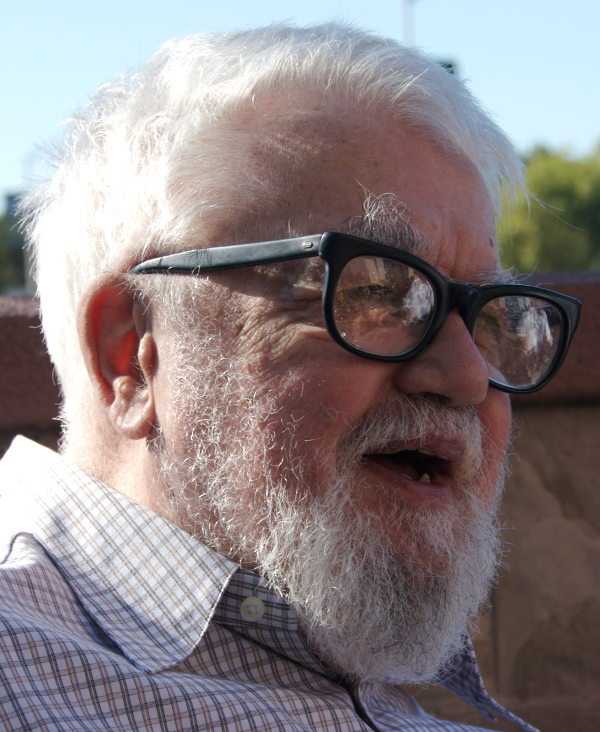
\includegraphics[width=1.2in]{img/john-mccarthy.png}
    \end{column}
    \begin{column}{0.7\textwidth}
      \begin{itemize}
        \item John McCarthy while at MIT -- late 1950s.
        \vspace{0.25cm}
        \item Created Lisp.
        \vspace{0.25cm}
        \item Lisp generally considered first functional programming language (not really though).
        \vspace{0.25cm}
        \item Lots of dialects exist today, such as Scheme and Common Lisp.
      \end{itemize}
    \end{column}
  \end{columns}
  \citeurl{www-formal.stanford.edu/jmc/}
\end{frame}

\begin{frame}[fragile]{Wasteful for loops}
  \begin{minted}[linenos, frame=lines, framesep=2mm]{python}
# How do you parallelise this?
inds = list(range(10))
total = 0
for i in inds:
  total = total + (i * 7)
  \end{minted}
  \begin{minted}[linenos, frame=lines, framesep=2mm]{python}
def byseven(i):
  return i * 7

inds = list(range(10))
sevens = map(byseven, inds)
total = sum(sevens)
  \end{minted}
\end{frame}

\begin{frame}{State}
\begin{description}
  \item[Imperative] programming is a programming paradigm where statements are used to change the \emph{state}.
  \item[State] is the name given to the current data/values related to an executing process, including internal stuff like the call stack.
  \item[Processes] begin with an initial state and (possibly) have (a number of) halt states.
  \item[Statements] change the state.
  \item[Functions] in imperative programming languages might return different values for the same input at different times, because of the state.
  \item[Functional] programming languages (try to) not depend on state.
\end{description}
\end{frame}


\begin{frame}{Side effects}
  \begin{description}
    \item[Functions] are said to have side effects if they modify the state (on top of returning a value).
    \item[Static and global] variables are often good examples of side effects in action.
    \item[Functional] programming tries to avoid side effects.
    \item[It's tricky] to avoid them -- such as when we need user input.
  \end{description}
\end{frame}

\begin{frame}[fragile]{Basic operators}
\begin{minted}[frame=lines, framesep=2mm]{scheme}
> (+ 3 4)
7
> (* 3 2)
6
> (- 5 3)
2
> (/ 6 3)
2
\end{minted}
\end{frame}

\begin{frame}[fragile]{More arguments}
\begin{minted}[frame=lines, framesep=2mm]{scheme}
> (+ 3 4 5)
(+ 3 4 5)
> (- 3 4 5)
-6
> (* 2 3 4)
24
> (/ 6 3 3)
2/3
> (/ 6 3 3 3)
2/9
\end{minted}
\end{frame}


\begin{frame}[fragile]{Functions and values}
\begin{minted}[frame=lines, framesep=2mm]{scheme}
; Define a value called foo with value 3.
>(define foo 3)

; Define a function f.	
>(define (f x)
  (+ (* 3 x) 12))

>(define (g x)
  (* 3 (+ x 4)))

>(g 2)
18
\end{minted}
\citeurl{www.artificialworlds.net/presentations/scheme-01-intro/scheme-01-intro.html}
\end{frame}

\begin{frame}[fragile]{Conditionals}
  \begin{minted}[frame=lines, framesep=2mm]{scheme}
> (if (< 1 2) '(y e s) '(n o))
(y e s)

>(define (abs x)
  (if (< x 0)
  (- x)
  x))

\end{minted}
\citeurl{www.artificialworlds.net/presentations/scheme-01-intro/scheme-01-intro.html}
\end{frame}


\begin{frame}[fragile]{Lists}
  \begin{minted}[frame=lines, framesep=2mm]{scheme}
>(list 1 2 3)
(1 2 3)

>(list 'a 'b 'c)
(a b c)

> (length (list 1 2 3))
3
\end{minted}
\citeurl{www.artificialworlds.net/presentations/scheme-01-intro/scheme-01-intro.html}
\end{frame}

\begin{frame}[fragile]{car and cdr}
  \begin{minted}[frame=lines, framesep=2mm]{scheme}
> (car (list 1 2 3))
1
> (cdr (list 1 2 3))
(2 3)
> (define l (list 1 2 3))
> (car l)
1
> (cdr l)
(2 3)
> (car (cdr l))
2
> (cadr l)
2
\end{minted}
\citeurl{www.artificialworlds.net/presentations/scheme-01-intro/scheme-01-intro.html}
\end{frame}

\begin{frame}[fragile]{Recursion}
  \begin{minted}[frame=lines, framesep=2mm]{scheme}
> (define (sum lv)              
    (if (null? lv)
      0
      (+ (car lv) (sum (cdr lv)))))
> (sum (list 1 2 3))                            
6
> (define (derange n)
    (if (= 0 n)
      '()
      (cons n (derange (- n 1)))))
> (derange 12)                                                    
(12 11 10 9 8 7 6 5 4 3 2 1)
\end{minted}
\citeurl{www.artificialworlds.net/presentations/scheme-01-intro/scheme-01-intro.html}
\end{frame}

\begin{frame}[fragile]{Looping recursively}
\begin{minted}[frame=lines, framesep=2mm]{scheme}
> (let loop ((i 5))
(print "i is " i ".\n")
(if (> i 0) (loop (- i 1))))
i is 5.
i is 4.
i is 3.
i is 2.
i is 1.
i is 0.
\end{minted}
\citeurl{gambitscheme.org/wiki/images/a/a7/A\_Tour\_of\_Scheme\_in\_Gambit.pdf}
\end{frame}

\begin{frame}[fragile]{Data and code}
\begin{minted}[frame=lines, framesep=2mm]{scheme}
> (define (swap3-1-2 x)
  (list (cadr x) (car x) (caddr x)))

> (swap3-1-2 (list 1 2 3))
(2 1 3)

> (define four-over-two (list 4 '/ 2))

> four-over-two
(4 / 2)

> (eval (swap3-1-2 four-over-two))
\end{minted}
\citeurl{www.artificialworlds.net/presentations/scheme-01-intro/scheme-01-intro.html}
\end{frame}

\begin{frame}[fragile]{More on functions}
\begin{minted}[frame=lines, framesep=2mm]{scheme}
; Printing stuff to terminal.
> (print "Ay" "-" "yo.\n")
; Proper way to define a function.
> (define foo (lambda (bar) (print "Bar is " bar ".\n")))
; Shorthand.
> (define (foo bar) (print "Bar is " bar ".\n"))

; Local variables.
> (define (foo bar) (let ((thing "Bar"))
    (print thing " is " bar ".\n")))
> (foo "open")
Bar is open.
\end{minted}
\citeurl{gambitscheme.org/wiki/images/a/a7/A\_Tour\_of\_Scheme\_in\_Gambit.pdf}
\end{frame}


\begin{frame}[fragile]{cons}
\begin{minted}[frame=lines, framesep=2mm]{scheme}
> (cons 1 '())
(1)
> (cons 1 (cons 2 null))
(1 2)
> (cons 1 (cons 2 (cons 3 null)))
(1 2 3)
> (define mylist (cons 1 (cons 2 (cons 3 null))))
> mylist
(1 2 3)
> (car mylist)
1
> (cdr mylist)
(2 3)
\end{minted}
\citeurl{www.artificialworlds.net/presentations/scheme-02-basics/scheme-02-basics.html}
\end{frame}

\begin{frame}[fragile]{More on lists}
\begin{minted}[frame=lines, framesep=2mm]{scheme}
> (list "a" "b" "c")
("a" "b" "c")
> (list a b c)
reference to undefined identifier: a
> (list 'a 'b 'c)
(a b c)

> (equal? 
(list 1 2 3)
(cons 1 (cons 2 (cons 3 '()))))
#t
\end{minted}
\citeurl{www.artificialworlds.net/presentations/scheme-02-basics/scheme-02-basics.html}
\end{frame}

\begin{frame}[fragile]{Quoting}
\begin{minted}[frame=lines, framesep=2mm]{scheme}
> (list a b c)
*** ERROR IN (console)@41.7 -- Unbound variable: a
> (quote (a b c))
(a b c)
> (quote a b c)
*** ERROR IN (console)@42.1 -- Ill-formed special form: quote
> '(a b c) 
(a b c)
> (define forty-two '(* 6 9))
> forty-two
(* 6 9)
> (eval forty-two)
54
\end{minted}
\citeurl{www.artificialworlds.net/presentations/scheme-05-quotation/scheme-05-quotation.html}
\end{frame}

\begin{frame}[fragile]{Null list}
\begin{minted}[frame=lines, framesep=2mm]{scheme}
> ()
missing procedure expression
> (list)
()
> '()
()
> null
()
> 'null
null
\end{minted}
\citeurl{www.artificialworlds.net/presentations/scheme-05-quotation/scheme-05-quotation.html}
\end{frame}

\begin{frame}[fragile]{Closures}
\begin{minted}[frame=lines, framesep=2mm]{scheme}
> (define (container value)
(lambda ()
(string-append "This container contains " value ".")))
> (define apple (container "an apple"))
> (define pie (container "a pie"))
> (apple)
"This container contains an apple."
> (apple)
"This container contains an apple."
> (pie)
"This container contains a pie."
\end{minted}
\citeurl{gambitscheme.org/wiki/images/a/a7/A\_Tour\_of\_Scheme\_in\_Gambit.pdf}
\end{frame}



\section{Turing Machines}

\section{Complexity Classes}
